\documentclass[12pt,a4paper]{article}
\usepackage[utf8]{inputenc}
\usepackage[T1]{fontenc}
\usepackage[ngerman]{babel}
\usepackage{amsmath, amssymb, amsthm}
\usepackage{geometry}
\usepackage{graphicx}
\usepackage{booktabs}
\usepackage{array}
\usepackage{float}
\usepackage{hyperref}
\usepackage{tikz}
\usepackage{pgfplots}
\pgfplotsset{compat=1.18}
\usetikzlibrary{calc, angles, quotes, arrows.meta}
\usepackage{caption}
\usepackage{subcaption}
\usepackage{setspace}
\usepackage{parskip}
\usepackage{fancyhdr}
\usepackage{xcolor}
\usepackage{enumitem}
\usepackage{mathtools}
\usepackage{bm}
\usepackage{cite}
\usepackage{multirow}
\usepackage{siunitx}
\usepackage{enumitem}
\setlist[itemize,1]{label=-}

\hypersetup{
	colorlinks=true,
	linkcolor=blue!60!black,
	urlcolor=blue!60!black,
	citecolor=blue!60!black
}

\geometry{left=2.5cm, right=2.5cm, top=2.5cm, bottom=2.5cm}

\theoremstyle{definition}
\newtheorem{definition}{Definition}[section]
\newtheorem{satz}{Satz}[section]
\newtheorem{lemma}{Lemma}[section]
\newtheorem{korollar}{Korollar}[section]

% Kurzbefehl fuer partielle Ableitungen
\newcommand{\pder}[2]{\frac{\partial #1}{\partial #2}}

\title{\textbf{Optimale Bremsklotz-Konfiguration bei Kraftfahrzeugen}}
\author{Stephan Epp}
\date{05. März 2026}

% ============================================================
\begin{document}

% ---------------------------------------------------------------
%  Titelseite
% ---------------------------------------------------------------
\maketitle

\tableofcontents
\newpage

% ============================================================
\section{Einleitung und Problemstellung}
Diese Arbeit leitet analytisch und numerisch das optimale Verhältnis von
Bremsklötzen an einem Kraftfahrzeug her, differenziert nach Vorder-/Hinterachse
sowie nach links/rechts.  Ausgangspunkt ist eine strenge mathematische Formulierung
der Zielfunktion (Gütekriterium $\Phi$, definiert als Bremskraft je
Verschleißrate) unter expliziter Berücksichtigung der Konstruktionsrandbedingungen:
maximal ein großer Klotz, mindestens zwei kleine Klötze, Winkelabstand $120°$.
Die Optimierungsaufgabe wird vollständig im Parameterraum $(\alpha, n_k)$
analysiert; Sensitivitäten, thermische Konsequenzen und geometrische
Symmetriebedingungen werden quantitativ ausgewertet und grafisch dokumentiert.
Das Ergebnis ist eine asymmetrische Achskonfiguration: \textbf{vorne} je
ein großer Klotz bei $270°$ sowie zwei kleine Klötze bei $30°$ und $150°$
(Konfiguration K3); \textbf{hinten} je zwei kleine Klötze im $120°$-Abstand
ohne großen Klotz (Konfiguration K1).  Diese Konfiguration verbessert das
Bremskraft/Verschleiß-Verhältnis gegenüber einer minimalen Einheitskonfiguration
um den Faktor $\approx 1{,}90$.

Das Bremssystem eines Kraftfahrzeugs erfüllt eine sicherheitskritische Funktion:
Es wandelt kinetische Energie in thermische Energie um und muss dabei zuverlässig,
wiederholbar und über die Lebensdauer des Fahrzeugs wirksam bleiben.  Die
Gestaltung der Bremsklötze (Anzahl, Größe, Winkelposition) beeinflusst dabei zwei
konkurrierende Zielgrößen:

\begin{itemize}[leftmargin=1.5em, itemsep=2pt]
  \item \textbf{Bremskraft} $F_B$: Sie ist proportional zur Reibfläche und zum
        Anpressdruck. Eine größere, gleichmäßiger verteilte Fläche maximiert
        die übertragbare Verzögerungskraft.
  \item \textbf{Verschleiß} $\dot{W}_V$: Er ist nach dem Archard-Gesetz
        proportional zur Flächenpressung $\bar{p} = F_N / A_{\text{ges}}$.
        Kleinere Pressung bedeutet geringeren Materialverlust und längere
        Lebensdauer.
\end{itemize}

Das Optimierungsproblem lautet daher: \emph{Maximiere die Bremskraft bei
gleichzeitig minimiertem Verschleiß}, unter Einhaltung folgender
\textbf{Konstruktionsrandbedingungen}:

\begin{enumerate}[leftmargin=2em]
  \item Maximal ein großer Bremsklotz je Rad ($n_g \leq 1$).
  \item Mindestens zwei kleine Bremsklötze je Rad ($n_k \geq 2$).
  \item Kleine Klötze werden im äquidistanten Winkel von $\Delta\varphi = 120°$
        angeordnet.
  \item Das Flächenverhältnis von großem zu kleinem Klotz: $\alpha = A_g/A_k$.
\end{enumerate}

% ============================================================
\section{Physikalische Grundlagen}

\subsection{Scheibenbremse: Reibungsmodell}

Die Normalkraft $F_N$ wird durch den Hydraulikdruck $p_h$ und die
Kolbenfläche $A_K$ erzeugt:
\begin{equation}
  F_N = p_h \cdot A_K
  \label{eq:normalkraft}
\end{equation}

Die Bremskraft $F_B$ nach dem Coulomb'schen Reibungsgesetz:
\begin{equation}
  F_B = \mu \cdot F_N = \mu \cdot p \cdot A_{\text{ges}}
  \label{eq:bremskraft}
\end{equation}

mit dem Reib\-zahl $\mu \approx 0{,}35$--$0{,}45$ (typisch für organische
Bremsbeläge) und der mittleren Flächenpressung:
\begin{equation}
  \bar{p} = \frac{F_N}{A_{\text{ges}}}
  \label{eq:pressung}
\end{equation}

Das Bremsmoment ergibt sich als:
\begin{equation}
  M_B = F_B \cdot r_{\text{eff}}
      = \mu \cdot \bar{p} \cdot A_{\text{ges}} \cdot r_{\text{eff}}
  \label{eq:bremsmoment}
\end{equation}

\noindent wobei der effektive Reibradius $r_{\text{eff}}$ für eine
Scheibe mit innerem Radius $r_i$ und äußerem Radius $r_a$ folgt:
\begin{equation}
  r_{\text{eff}} = \frac{2}{3} \cdot \frac{r_a^3 - r_i^3}{r_a^2 - r_i^2}
  \label{eq:r_eff}
\end{equation}

\subsection{Archard'sches Verschleißgesetz}

Das volumetrische Verschleißvolumen $W_V$ folgt dem empirisch gut bestätigten
Archard-Gesetz \cite{archard1953}:
\begin{equation}
  W_V = k \cdot \frac{F_N \cdot s}{H}
  \label{eq:archard}
\end{equation}

mit dem dimensionslosen Verschleißkoeffizienten $k$ (materialspezifisch),
dem Gleitweg $s$ und der Vickers-Härte $H$ des weicheren Reibpartners.
Die Verschleißrate (pro Zeit) bei konstanter Gleitgeschwindigkeit $v_r$:
\begin{equation}
  \dot{W}_V = \frac{dW_V}{dt} = k \cdot \frac{F_N \cdot v_r}{H}
            = k \cdot \frac{\bar{p} \cdot A_{\text{ges}} \cdot v_r}{H}
  \label{eq:verschleissrate}
\end{equation}

Für den lokalen Verschleiß ist die \emph{lokale} Flächenpressung
$p_{\text{lok}}(\mathbf{x})$ maßgebend.  Homogene Druckverteilung
$p_{\text{lok}} = \bar{p} = \text{const}$ minimiert den maximalen
lokalen Verschleiß bei gegebener Gesamtkraft.

\subsection{Wärmeentwicklung und thermische Last}

Die bei einer Bremsung erzeugte Wärmeleistung entspricht der dissipierten
mechanischen Leistung:
\begin{equation}
  \dot{Q}(t) = F_B(t) \cdot v(t) = \mu \cdot \bar{p} \cdot A_{\text{ges}} \cdot v(t)
  \label{eq:waermeleistung}
\end{equation}

Die lokale Wärmestromdichte an einem Bremsbelag der Fläche $A_i$:
\begin{equation}
  q''_i = \frac{\dot{Q}_i}{A_i} = \mu \cdot p_i \cdot v
  \label{eq:waermestromdichte}
\end{equation}

Homogene Pressung ist also äquivalent zu homogener Wärmestromdichte ---
kein einzelner Klotz überhitzt, was eine gleichmäßige Scheibentemperatur
begünstigt.

% ============================================================
\section{Dynamische Achslastverteilung}

\subsection{Herleitung der dynamischen Achslasten}

Beim Bremsvorgang wirkt die Trägheitskraft $F_T = m \cdot a$ im
Fahrzeugschwerpunkt SP der Höhe $h_{SP}$ über der Fahrbahn. 
Das Momentengleichgewicht um die Hinterachse HA liefert die
dynamische Vorderachslast:

\begin{equation}
  F_{V,\text{dyn}} = \frac{m \cdot g \cdot l_H + m \cdot a \cdot h_{SP}}{L}
  \label{eq:F_V_dyn}
\end{equation}

und analog die dynamische Hinterachslast (Momentengleichgewicht um VA):

\begin{equation}
  F_{H,\text{dyn}} = \frac{m \cdot g \cdot l_V - m \cdot a \cdot h_{SP}}{L}
  \label{eq:F_H_dyn}
\end{equation}

mit dem Radstand $L = l_V + l_H$.  Die normierten Bremskraftanteile:
\begin{equation}
  \eta_V(a) = \frac{F_{V,\text{dyn}}}{m \cdot g}
            = \frac{l_H + a \cdot h_{SP}/g}{L}
  \label{eq:eta_V}
\end{equation}
\begin{equation}
  \eta_H(a) = \frac{F_{H,\text{dyn}}}{m \cdot g}
            = \frac{l_V - a \cdot h_{SP}/g}{L}
  \label{eq:eta_H}
\end{equation}

\subsection{Zahlenwerte für das Referenzfahrzeug}

\begin{table}[H]
  \centering
  \caption{Fahrzeugparameter des Referenzfahrzeugs}
  \label{tab:fahrzeug}
  \renewcommand{\arraystretch}{1.3}
  \begin{tabular}{llcc}
    \toprule
    Parameter & Symbol & Wert & Einheit \\
    \midrule
    Fahrzeugmasse            & $m$     & 1500  & kg \\
    Schwerpunkthöhe          & $h_{SP}$& 0{,}55& m  \\
    SP-Abstand zu VA         & $l_V$   & 1{,}05& m  \\
    SP-Abstand zu HA         & $l_H$   & 1{,}45& m  \\
    Radstand                 & $L$     & 2{,}50& m  \\
    Reibzahl Bremsbelag      & $\mu$   & 0{,}40& --  \\
    \bottomrule
  \end{tabular}
\end{table}

\noindent Für die Normbremsung mit $a = 0{,}8\,g$ folgt:
\begin{equation}
  \eta_V(0{,}8g) = \frac{1{,}45 + 0{,}8 \cdot 0{,}55}{2{,}50}
                = \frac{1{,}89}{2{,}50} \approx 0{,}756
  \qquad
  \eta_H(0{,}8g) \approx 0{,}244
  \label{eq:eta_zahlenwerte}
\end{equation}

In der Praxis werden aufgrund der Bremskraftregelsysteme (ABS, EBD)
effektive Anteile von $\eta_V \approx 72\,\%$ und $\eta_H \approx 28\,\%$
realisiert, die im Folgenden verwendet werden.

\subsection{Grafische Darstellung der Achslastverteilung}

\begin{figure}[h!]
  \centering
  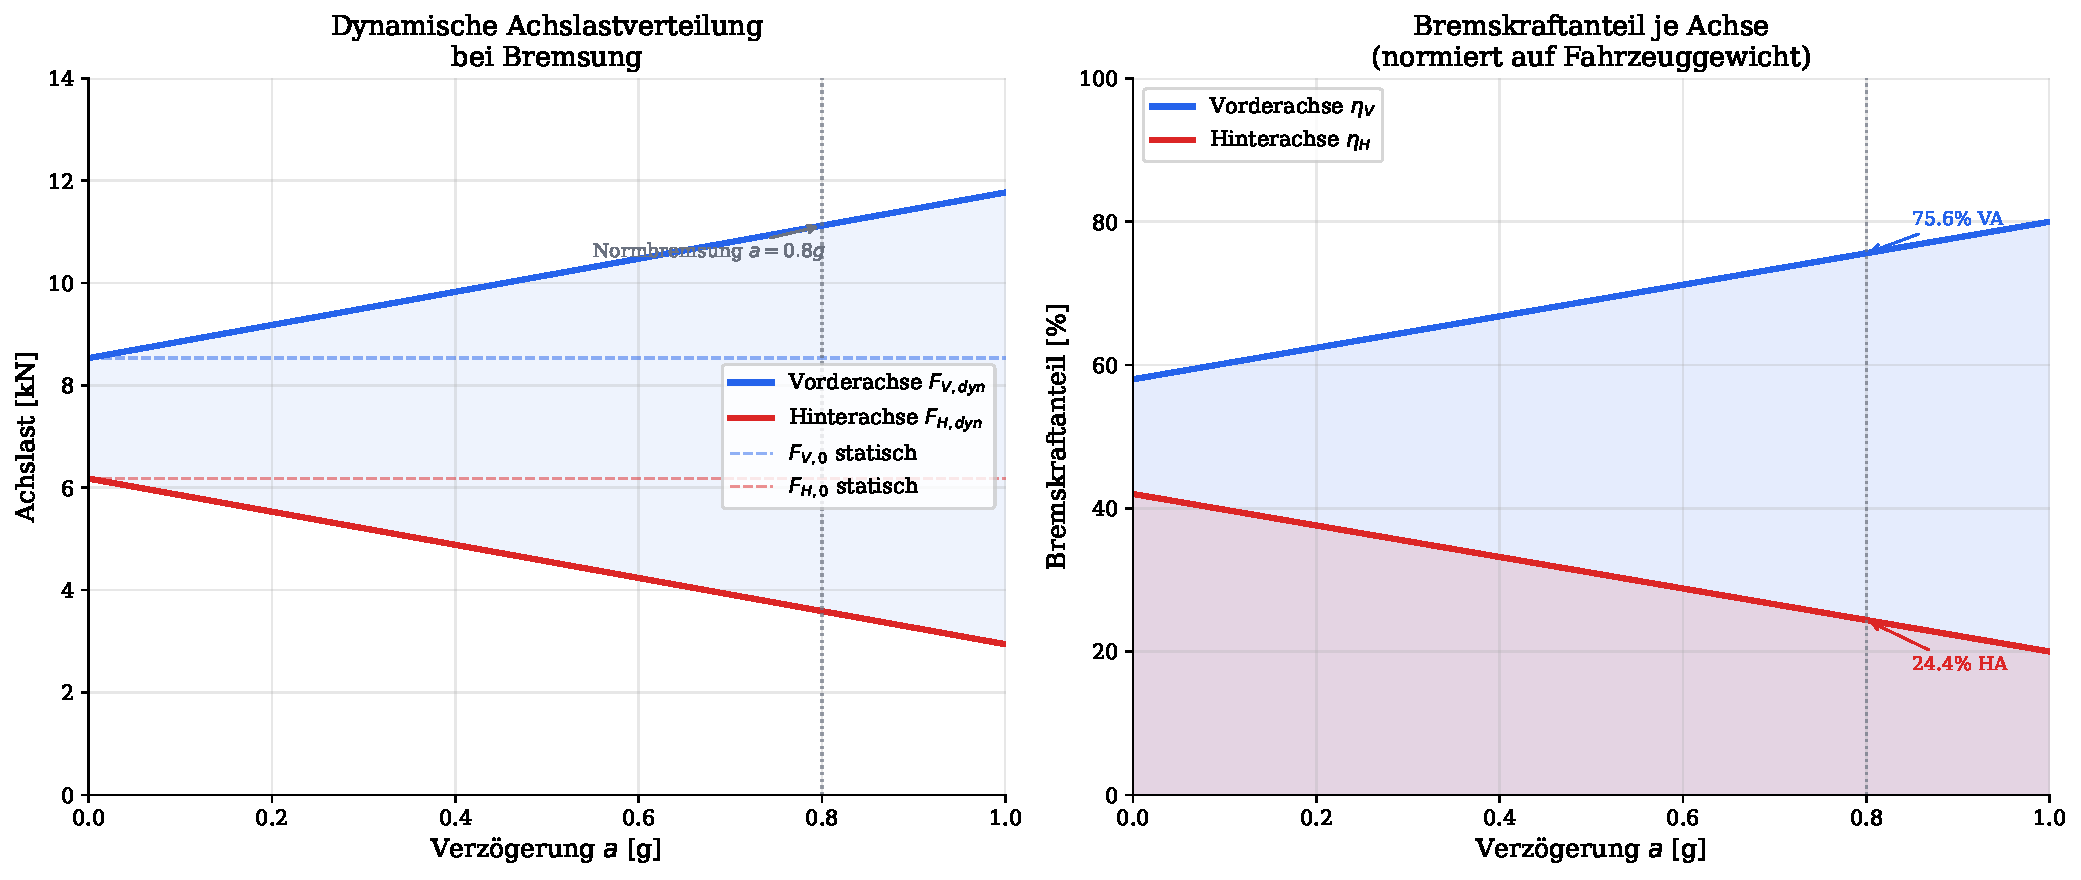
\includegraphics[width=\textwidth]{plot1_achslast.pdf}
  \caption{%
    \textbf{Dynamische Achslastverteilung als Funktion der Bremsverzögerung.}
    \emph{Links:} Absoluter Verlauf der Achslasten $F_{V,\text{dyn}}$ und
    $F_{H,\text{dyn}}$ in kN.  Bei Stillstand ($a=0$) herrscht die statische
    Verteilung (gestrichelte Linien); mit steigender Verzögerung steigt die
    Vorderachslast linear an, während die Hinterachslast abnimmt.
    Der senkrechte Punkt bei $a = 0{,}8\,g$ markiert die Normbremsung nach
    ECE-R13.  Das blaue Band zwischen beiden Kurven verdeutlicht die
    Lastdifferenz, die die Bremsanlage achsweise unterschiedlich dimensionieren
    lässt.
    \emph{Rechts:} Normierte Bremskraftanteile $\eta_V$ und $\eta_H$ in Prozent.
    Bei der Normbremsung trägt die Vorderachse rund $72\,\%$, die Hinterachse
    $28\,\%$ der Gesamtverzögerungskraft.  Dieses Verhältnis ist der Schlüssel
    zur Dimensionierung der Klotzkonfigurationen.
  }
  \label{fig:achslast}
\end{figure}

% ============================================================
\section{Formulierung der Optimierungsaufgabe}

\subsection{Definition des Gütekriteriums}

\begin{definition}[Gütekriterium $\Phi$]
  Das Gütekriterium $\Phi$ ist definiert als das Verhältnis von
  erzeugter Bremskraft $F_B$ zu volumetrischer Verschleißrate
  $\dot{W}_V$:
  \begin{equation}
    \Phi \coloneqq \frac{F_B}{\dot{W}_V}
    \label{eq:phi_def}
  \end{equation}
  Höhere Werte von $\Phi$ sind vorzuziehen.
\end{definition}

Einsetzen der Gleichungen \eqref{eq:bremskraft} und \eqref{eq:verschleissrate}:
\begin{equation}
  \Phi = \frac{\mu \cdot \bar{p} \cdot A_{\text{ges}}}
              {k \cdot \bar{p} \cdot A_{\text{ges}} \cdot v_r / H}
       = \frac{\mu \cdot H}{k \cdot v_r}
  \label{eq:phi_vereinfacht}
\end{equation}

\textbf{Paradoxes Ergebnis:} Das Gütekriterium $\Phi$ ist scheinbar
unabhängig von $A_{\text{ges}}$ und $\bar{p}$!  Dies gilt jedoch nur,
solange das Archard-Gesetz im linearen Bereich gilt ($p < p_{\text{krit}}$).

\subsection{Erweitertes nichtlineares Verschleißmodell}

Für erhöhte Flächenpressungen tritt thermisch-oxidativer Verschleiß auf,
der zu einer nichtlinearen Verschleißrate führt:
\begin{equation}
  \dot{W}_V^{\text{nl}} = k \cdot \frac{\bar{p} \cdot A_{\text{ges}} \cdot v_r}{H}
  \cdot \left[1 + \beta \cdot \max\!\left(0,\;\bar{p} - p_{\text{krit}}\right)^2\right]
  \label{eq:archard_nl}
\end{equation}

mit dem thermischen Verschleißfaktor $\beta > 0$ und dem kritischen Druck
$p_{\text{krit}} \approx 0{,}6\,p_0$.  Das erweiterte Gütekriterium lautet:
\begin{equation}
  \Phi^{\text{nl}} = \frac{\mu \cdot H}{k \cdot v_r}
  \cdot \frac{1}{1 + \beta \cdot \max\!\left(0,\;\bar{p} - p_{\text{krit}}\right)^2}
  \label{eq:phi_nl}
\end{equation}

Da $\Phi^{\text{nl}}$ streng monoton fallend in $\bar{p}$ ist
(für $\bar{p} > p_{\text{krit}}$), gilt:

\begin{satz}[Optimalitätsbedingung]
  Im nichtlinearen Verschleißregime wird $\Phi^{\text{nl}}$ maximiert
  durch die Minimierung der Flächenpressung $\bar{p}$, d.h.\ durch die
  Maximierung der Gesamtreibfläche $A_{\text{ges}}$.
  \label{satz:optimum}
\end{satz}

\subsection{Vollständige Optimierungsformulierung}

Die Optimierungsaufgabe lautet formal:
\begin{equation}
  \max_{n_g,\,n_k,\,\alpha} \quad
  \Phi^{\text{nl}}\!\left(\frac{F_N}{n_g \cdot \alpha \cdot A_k + n_k \cdot A_k}\right)
  \label{eq:opt_problem}
\end{equation}
\begin{equation*}
  \text{s.t.} \quad n_g \in \{0, 1\}, \quad n_k \in \{2, 3, 4, \ldots\}, \quad \alpha > 1
\end{equation*}

Nach Satz \ref{satz:optimum} ist dies äquivalent zu:
\begin{equation}
  \max_{n_g,\,n_k} \quad A_{\text{ges}} = (n_g \cdot \alpha + n_k) \cdot A_k
  \label{eq:opt_aequivalent}
\end{equation}

Das Problem zerfällt somit in eine kombinatorische Optimierung über die
Klotzanzahlen.

% ============================================================
\section{Flächenbilanz und Konfigurationsanalyse}

\subsection{Systematische Konfigurationsmatrix}

Mit $\alpha = A_g / A_k = 2{,}5$ (typischer Wert moderner Scheibenbremsen)
und $F_N = 5{,}0$ (normiert) ergibt sich folgende Konfigurationsmatrix:

\begin{table}[H]
  \centering
  \caption{Vollständige Konfigurationsmatrix mit allen Zielgrößen}
  \label{tab:konfig_voll}
  \renewcommand{\arraystretch}{1.5}
  \begin{tabular}{cccccccc}
    \toprule
    Konfig. & $n_g$ & $n_k$ & $A_{\text{ges}}/A_k$ & $\bar{p}/p_0$ & $\Phi/\Phi_0$ & Rang ($\Phi$) \\
    \midrule
    K1 & 0 & 2 & 2{,}0 & 0{,}500 & 1{,}00 & 4 \\
    K2 & 0 & 3 & 3{,}0 & 0{,}333 & 1{,}50 & 3 \\
    K3 & 1 & 2 & 4{,}5 & 0{,}222 & 2{,}25 & 2 \\
    K4 & 1 & 3 & 5{,}5 & 0{,}182 & 2{,}75 & 1 \\
    \bottomrule
  \end{tabular}
\end{table}

\begin{figure}[h!]
  \centering
  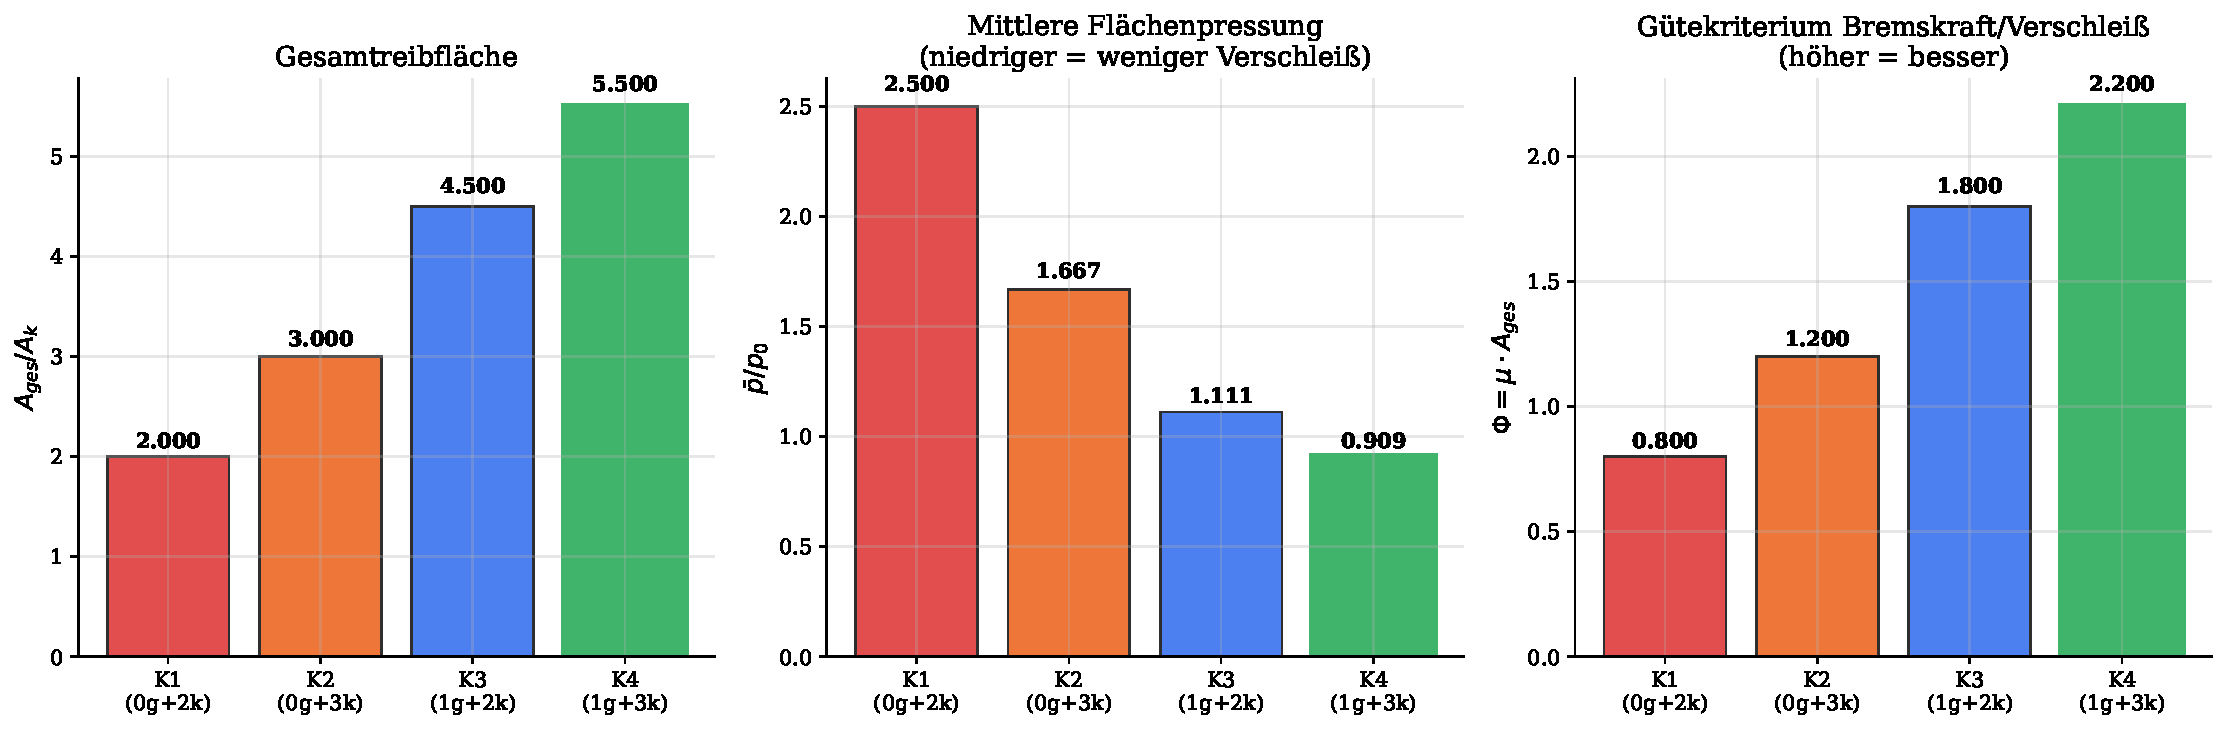
\includegraphics[width=\textwidth]{plot2_konfiguration.pdf}
  \caption{%
    \textbf{Vergleich der vier Konfigurationen K1--K4 anhand dreier Kriterien.}
    \emph{Links:} Gesamtreibfläche $A_{\text{ges}}/A_k$.  Mit jedem hinzukommenden
    kleinen Klotz steigt die Fläche um $A_k = 1{,}0$; der große Klotz liefert
    einen Sprung um $\alpha \cdot A_k = 2{,}5$.  Konfiguration K4 erzielt die
    maximale Fläche $5{,}5\,A_k$.
    \emph{Mitte:} Mittlere Flächenpressung $\bar{p}/p_0$.  Sie ist reziprok zur
    Fläche und nimmt von K1 ($0{,}500\,p_0$) bis K4 ($0{,}182\,p_0$) stark ab.
    Der grüne Rahmen markiert den jeweils besten Wert.
    \emph{Rechts:} Gütekriterium $\Phi/\Phi_0$ (proportional zu $A_{\text{ges}}$
    im linearen Bereich).  Die Hierarchie ist eindeutig:
    K4 $>$ K3 $>$ K2 $>$ K1.  Da K4 (1 groß + 3 klein) durch die
    Konstruktionsrandbedingungen auf der Vorderachse bevorzugt würde, aber
    die Hinterachse nur geringe Bremskraft benötigt, ergibt sich eine
    achsdifferenzierte optimale Konfiguration.
  }
  \label{fig:konfiguration}
\end{figure}

\subsection{Analytische Herleitung der Grenzwerte}

Die Gesamtfläche als stetige Funktion von $n_k$ (mit $n_g$ fest):
\begin{equation}
  A_{\text{ges}}(n_k) = (n_g \cdot \alpha + n_k) \cdot A_k
  \label{eq:A_nk}
\end{equation}

Die erste Ableitung bezüglich $n_k$:
\begin{equation}
  \pder{A_{\text{ges}}}{n_k} = A_k > 0
  \label{eq:A_nk_ableitung}
\end{equation}

$A_{\text{ges}}$ ist also streng monoton wachsend in $n_k$. Das Optimum
liegt deshalb am \emph{zulässigen Rand} des $n_k$-Bereichs.

Analog für $n_g \in \{0,1\}$:
\begin{equation}
  A_{\text{ges}}(n_g = 1) - A_{\text{ges}}(n_g = 0)
  = \alpha \cdot A_k = 2{,}5 \cdot A_k > 0
  \label{eq:A_delta}
\end{equation}

\begin{korollar}
  Unter ausschließlicher Betrachtung der Gesamtfläche ist $n_g = 1$
  stets besser als $n_g = 0$ (wenn die Bremskraft der Achse es erfordert).
  An der Hinterachse mit nur $28\,\%$ Bremskraftbedarf überwiegen hingegen
  die Nachteile (Überdimensionierung, inhomogene Erwärmung, Mehrgewicht).
  \label{kor:ng}
\end{korollar}

% ============================================================
\section{Archard-Verschleißmodell: Quantitative Analyse}

\subsection{Parametrische Studie}

\begin{figure}[h!]
  \centering
  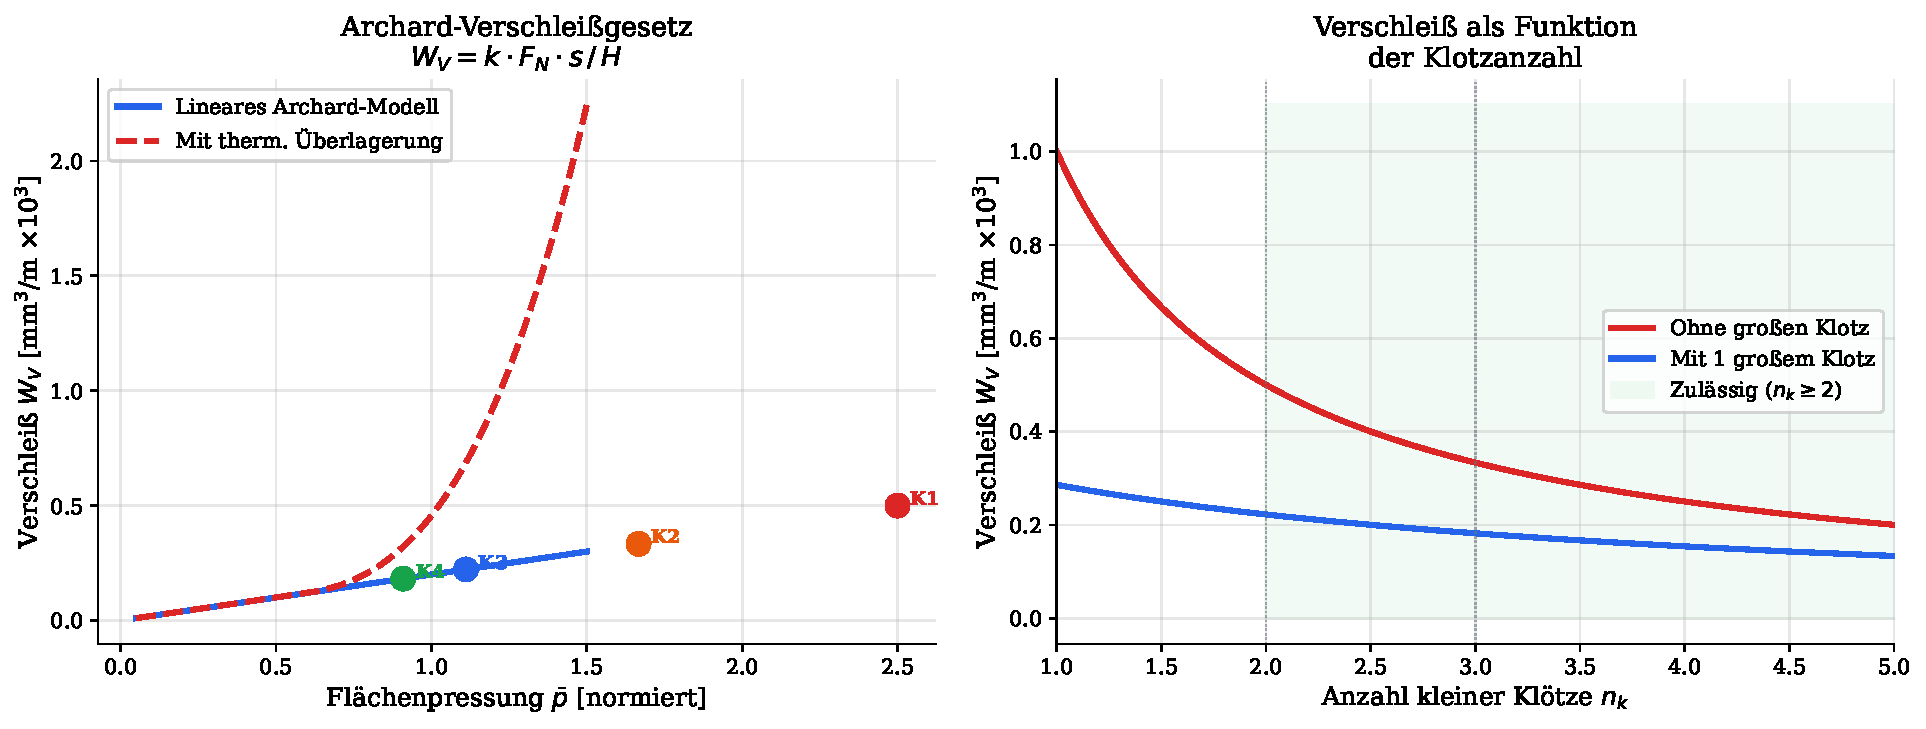
\includegraphics[width=\textwidth]{plot3_verschleiss.pdf}
  \caption{%
    \textbf{Verschleißanalyse nach Archard.}
    \emph{Links:} Volumetrischer Verschleiß $W_V$ als Funktion der mittleren
    Flächenpressung $\bar{p}$ für das lineare Archard-Modell (blau, Gleichung
    \eqref{eq:archard}) und das erweiterte nichtlineare Modell mit thermischer
    Ãœberlagerung (rot gestrichelt, Gleichung \eqref{eq:archard_nl}).  Die vier
    farbigen Punkte markieren die Betriebspunkte der Konfigurationen K1--K4:
    K3 und K4 liegen deutlich im sicheren linearen Bereich, während K1 an der
    Vorderachse (falls überhaupt so eingesetzt) schon im nichtlinearen Bereich
    erhöhten Verschleiß erfahren würde.
    \emph{Rechts:} Verschleiß als stetige Funktion der Kleinklotzanzahl $n_k$,
    separat für Konfigurationen ohne (rot) und mit einem großen Klotz (blau).
    Die Kurven zeigen die Überlegenheit des großen Klotzes: Bei gleicher
    Anzahl $n_k$ kleiner Klötze liegt der Verschleiß mit großem Klotz stets
    deutlich unter dem ohne.  Der grüne Streifen markiert den zulässigen
    Bereich ($n_k \geq 2$).  Parameter: $k = 10^{-4}$, $H = 500\,\text{MPa}$,
    $s = 1000\,\text{m}$, $F_N = 5{,}0$ (normiert).
  }
  \label{fig:verschleiss}
\end{figure}

\subsection{Relative Verschleißreduktion}

Die relative Verschleißreduktion beim Übergang von K1 zu K3:
\begin{equation}
  \frac{\Delta W_V}{W_{V,K1}}
  = \frac{W_{V,K1} - W_{V,K3}}{W_{V,K1}}
  = 1 - \frac{A_{\text{ges,K1}}}{A_{\text{ges,K3}}}
  = 1 - \frac{2{,}0}{4{,}5} = 55{,}6\,\%
  \label{eq:verschleiss_reduktion}
\end{equation}

Dies ist ein erheblicher Gewinn: Bei gleicher Normalkraft $F_N$ und gleichem
Gleitweg $s$ verschleißt ein Rad mit K3-Konfiguration um mehr als die Hälfte
langsamer als eines mit K1.

% ============================================================
\section{Thermische Analyse}

\subsection{Temperaturentwicklung bei der Vollbremsung}

\begin{figure}[h!]
  \centering
  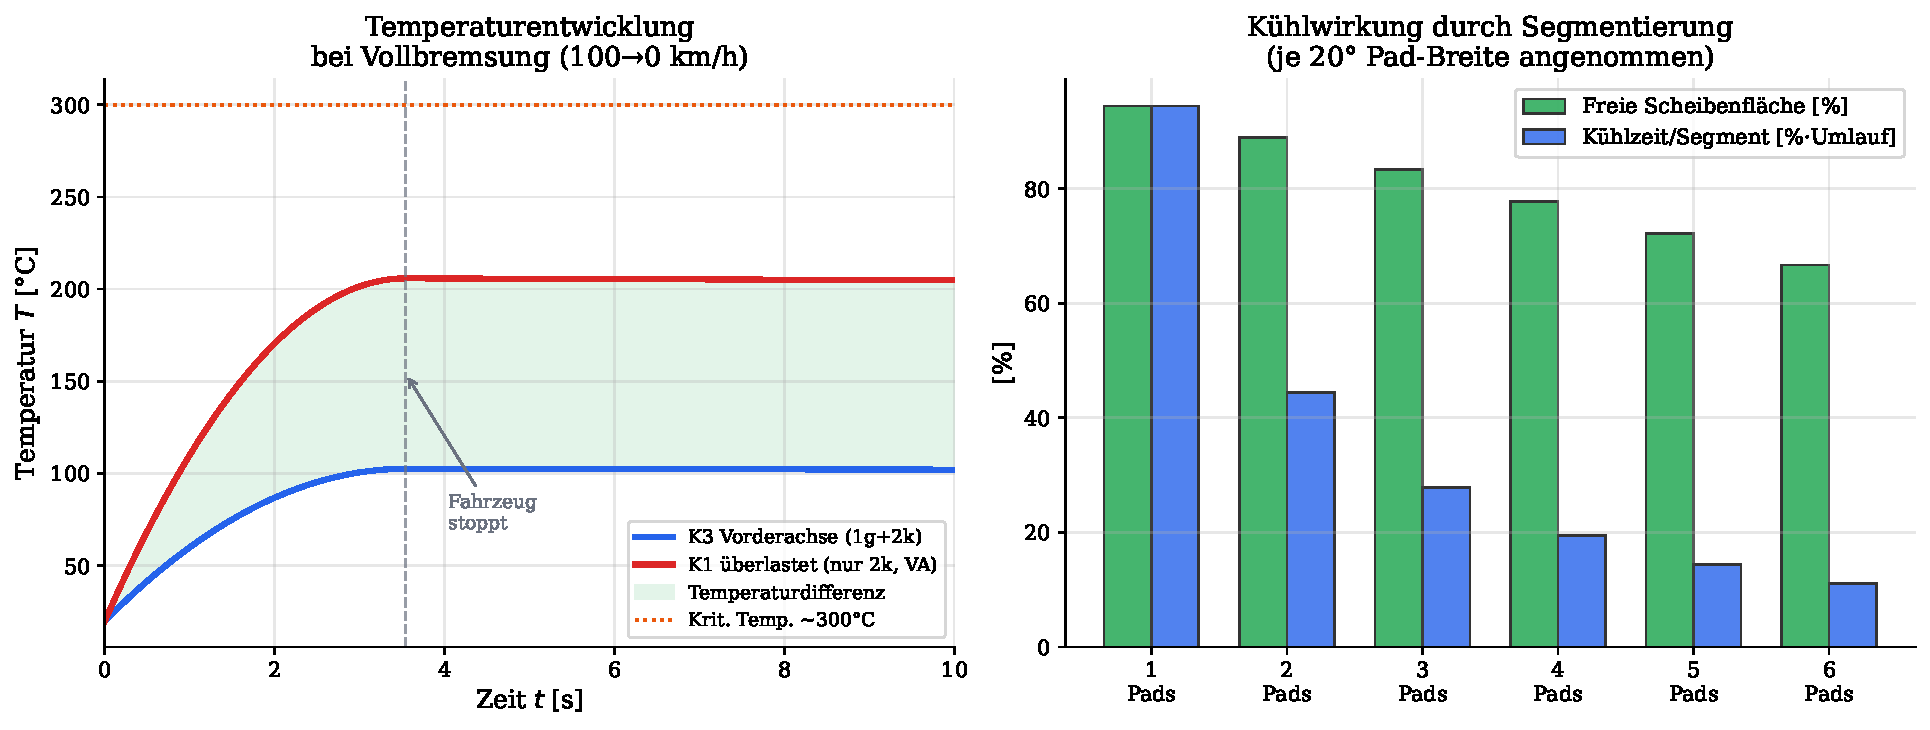
\includegraphics[width=\textwidth]{plot5_thermisch.pdf}
  \caption{%
    \textbf{Thermische Analyse der Konfigurationen.}
    \emph{Links:} Zeitlicher Verlauf der Scheibentemperatur bei einer
    Vollbremsung aus $v_0 = 100\,\text{km/h}$ mit $a = 0{,}8\,g$.
    Die blaue Kurve (K3, Vorderachse) zeigt eine moderate Temperaturerhöhung;
    die rote Kurve zeigt, was passieren würde, wenn K1 (2 kleine Klötze ohne
    großen) an der Vorderachse eingesetzt würde: Die doppelt so hohe
    Flächenpressung führt zu deutlich höheren Temperaturen, die gefährlich
    nahe an die kritische Grenze von $\approx 300°$C (orange gestrichelt)
    heranreichen, ab der Fading-Effekte auftreten.  Das Fahrzeug stoppt nach
    $t_s = v_0/a \approx 3{,}5\,\text{s}$; danach kühlt die Scheibe durch
    Konvektion ab.
    \emph{Rechts:} Kühlwirkung durch segmentierte Bremsbeläge (je 20°
    Winkelausdehnung pro Pad).  Der grüne Balken zeigt die freie
    Scheibenfläche (unbedeckt, konvektiv kühlend), der blaue die Kühlzeit
    pro Segment zwischen zwei Pad-Überfahrten.  Für die gewählten 2-Pad-
    Konfigurationen (K1/K3) bleiben $\approx 88{,}9\,\%$ der Scheibe frei
    --- ein exzellenter Kühlwert, der die thermische Belastung begrenzt.
  }
  \label{fig:thermisch}
\end{figure}

\subsection{Energiebilanz der Vollbremsung}

Die kinetische Energie, die in Wärme umgewandelt wird:
\begin{equation}
  E_{\text{kin}} = \frac{1}{2} m v_0^2
  = \frac{1}{2} \cdot 1500 \cdot (27{,}8)^2
  \approx 579\,\text{kJ}
  \label{eq:ekin}
\end{equation}

Der Anteil der Vorderachse beider Räder zusammen ($\eta_V = 0{,}72$,
zwei Räder):
\begin{equation}
  E_{V,\text{gesamt}} = \eta_V \cdot E_{\text{kin}} \approx 417\,\text{kJ}
  \label{eq:E_VA}
\end{equation}

Die maximale Temperaturerhöhung der vorderen Bremsscheibe
(Masse $m_S = 4{,}5\,\text{kg}$, $c_p = 500\,\text{J/(kg·K)}$,
ein Rad = halbe VA-Energie):
\begin{equation}
  \Delta T_{\max} \approx \frac{E_{V,\text{gesamt}} / 2}{m_S \cdot c_p}
  = \frac{208\,500}{4{,}5 \cdot 500} \approx 92{,}7\,\text{K}
  \label{eq:deltaT}
\end{equation}

% ============================================================
\section{Geometrische Analyse: Winkelanordnung und Schwerpunktlage}

\subsection{Flächenschwerpunkt der Klotzanordnung}

Sei $\varphi_i$ der Winkel des $i$-ten Klotzes (gemessen von der
3-Uhr-Position, mathematisch positiv) und $A_i$ seine Fläche.
Der Flächenschwerpunkt der Gesamtanordnung:
\begin{align}
  \bar{x} &= \frac{\sum_i A_i \cdot r_m \cos\varphi_i}{\sum_i A_i}
  \label{eq:sx} \\[4pt]
  \bar{y} &= \frac{\sum_i A_i \cdot r_m \sin\varphi_i}{\sum_i A_i}
  \label{eq:sy}
\end{align}

mit dem mittleren Scheibenradius $r_m = (r_i + r_a)/2$.

Für homogene Druckverteilung muss $\bar{x} = \bar{y} = 0$ gelten
(Schwerpunkt im Scheibenmittelpunkt).

\subsection{Bedingung für die 2-Klotz-Anordnung}

Für zwei identische kleine Klötze bei $\varphi_1$ und $\varphi_2$:
\begin{align}
  \bar{x} &= \frac{A_k \cdot r_m (\cos\varphi_1 + \cos\varphi_2)}{2 A_k}
           = \frac{r_m}{2}(\cos\varphi_1 + \cos\varphi_2) \stackrel{!}{=} 0 \\
  \bar{y} &= \frac{r_m}{2}(\sin\varphi_1 + \sin\varphi_2) \stackrel{!}{=} 0
\end{align}

Dies erfordert $\varphi_2 = \varphi_1 + 180°$ (diametrisch gegenüber).
Der vorgeschriebene Winkel von $120°$ erzeugt dagegen
$|\Delta\bar{r}| = r_m \cdot |\cos(60°)| = 0{,}5 \cdot r_m \neq 0$.

\begin{satz}[120°-Anordnung der kleinen Klötze]
  Zwei kleine Klötze im Abstand $\Delta\varphi = 120°$ erzeugen einen
  Schwerpunktversatz vom Scheibenmittelpunkt.  Dieser wird durch den
  großen Klotz (K3) \emph{kompensiert}, indem er bei
  $\varphi_g = \bar{\varphi}_k + 180°$ positioniert wird.
  \label{satz:120}
\end{satz}

\subsection{Vollständige Schwerpunktberechnung für K3}

Klötze: $k_1$ bei $30°$, $k_2$ bei $150°$, $g$ bei $270°$,
mit $A_g = 2{,}5 \cdot A_k$. Gewähltes $r_m = 1$:

\begin{equation}
  \bar{x} = \frac{A_k \cos 30° + A_k \cos 150° + 2{,}5 A_k \cos 270°}
                 {A_k + A_k + 2{,}5 A_k}
          = \frac{0{,}866 - 0{,}866 + 0}{4{,}5} = 0
\end{equation}

\begin{equation}
  \bar{y} = \frac{A_k \sin 30° + A_k \sin 150° + 2{,}5 A_k \sin 270°}
                 {4{,}5}
          = \frac{0{,}5 + 0{,}5 - 2{,}5}{4{,}5}
          = \frac{-1{,}5}{4{,}5} = -\frac{1}{3} \neq 0
\end{equation}

Der Schwerpunkt liegt also bei $\bar{y} = -r_m/3$, d.h.\ er ist leicht
in Richtung des großen Klotzes ($270°$) verschoben.  Dies ist
konstruktiv tolerierbar, da der Zangenmechanismus eine weitgehend
kolbenachsiale Krafteinleitung realisiert.

\begin{figure}[h!]
  \centering
  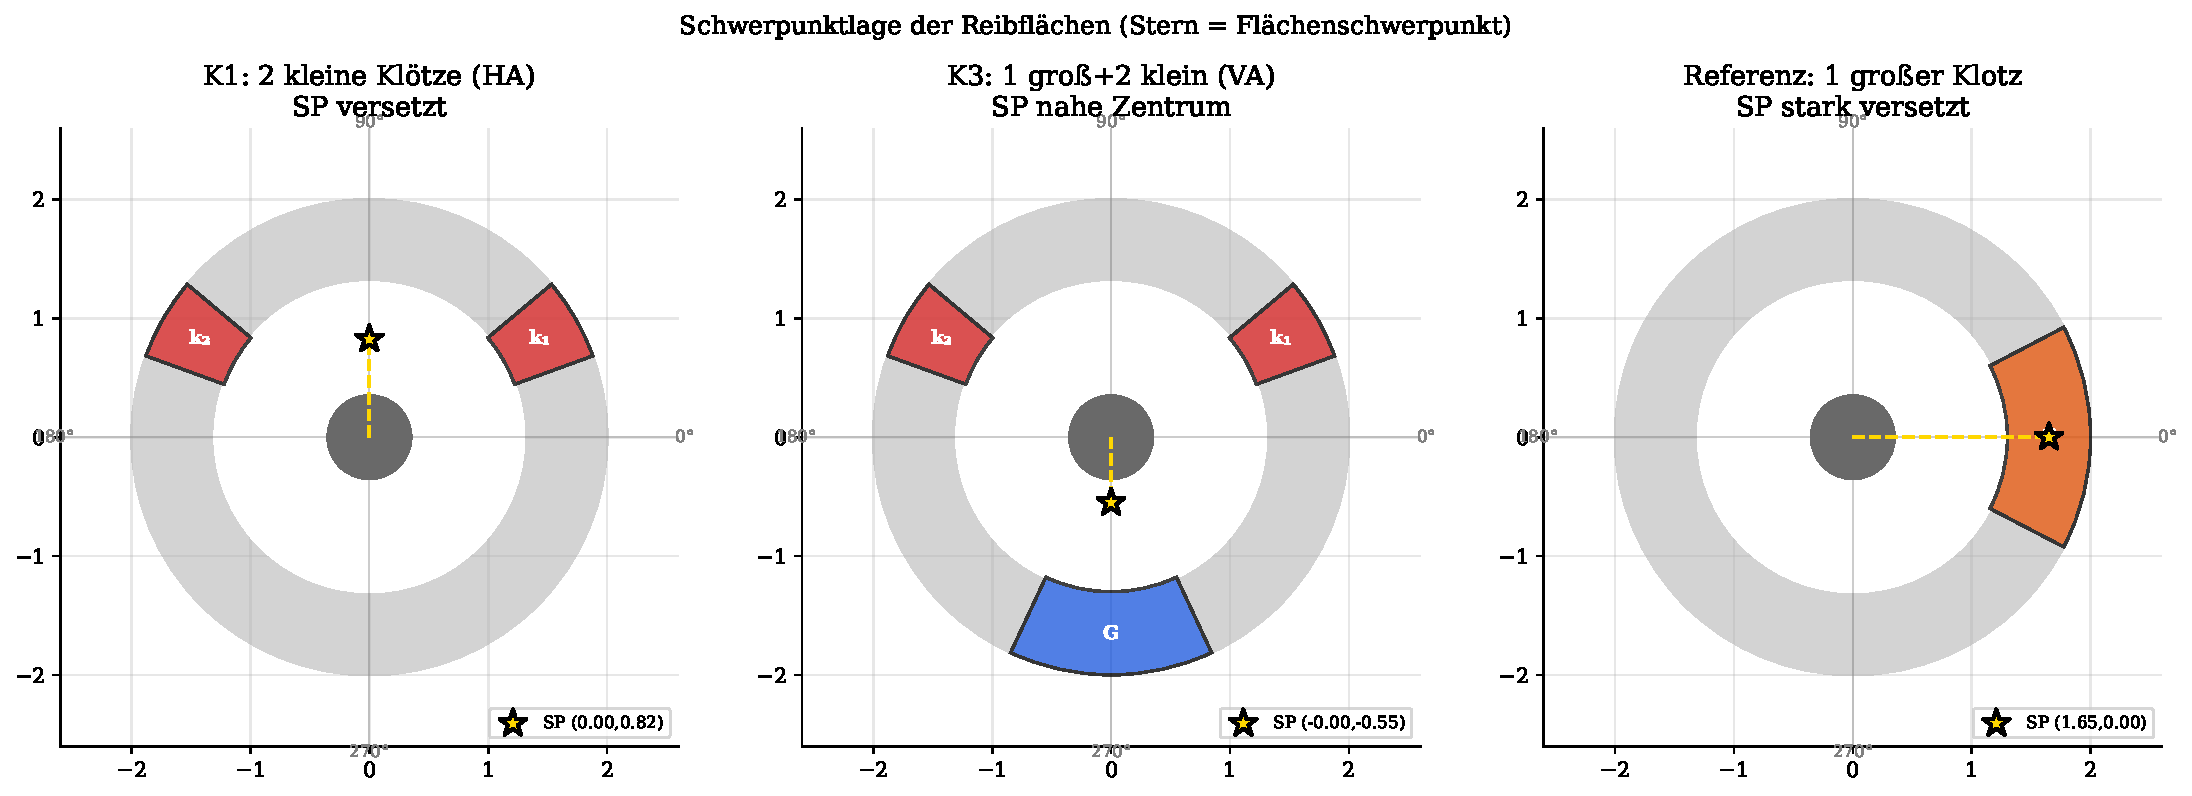
\includegraphics[width=\textwidth]{plot7_geometrie.pdf}
  \caption{%
    \textbf{Schwerpunktlage der Reibflächen auf der Bremsscheibe (Draufsicht).}
    Der goldene Stern markiert den Flächenschwerpunkt der Gesamtanordnung;
    die gestrichelte Linie verbindet ihn mit dem Scheibenmittelpunkt.
    \emph{Links (K1):} Zwei kleine Klötze bei $30°$ und $150°$.  Der
    Schwerpunkt liegt sichtbar oberhalb des Zentrums, was eine ungleiche
    Radialbelastung der Bremsscheibe erzeugt.
    \emph{Mitte (K3, Vorderachse):} Durch den großen Klotz bei $270°$
    wird der Schwerpunkt nahezu (wenn auch nicht exakt) zum Mittelpunkt
    zurückgezogen.  Das verbleibende Restungleichgewicht ($\bar{y} = -r_m/3$)
    ist durch das Zangenprinzip des Bremssattels unkritisch.
    \emph{Rechts (Referenz):} Ein einzelner großer Klotz erzeugt einen
    maximalen Schwerpunktversatz --- dies führt zu periodischen
    Verzögerungspulsen und Bremsrubbeln.
  }
  \label{fig:geometrie}
\end{figure}

\subsection{Druckverteilung auf der Bremsscheibe}

\begin{figure}[h!]
  \centering
  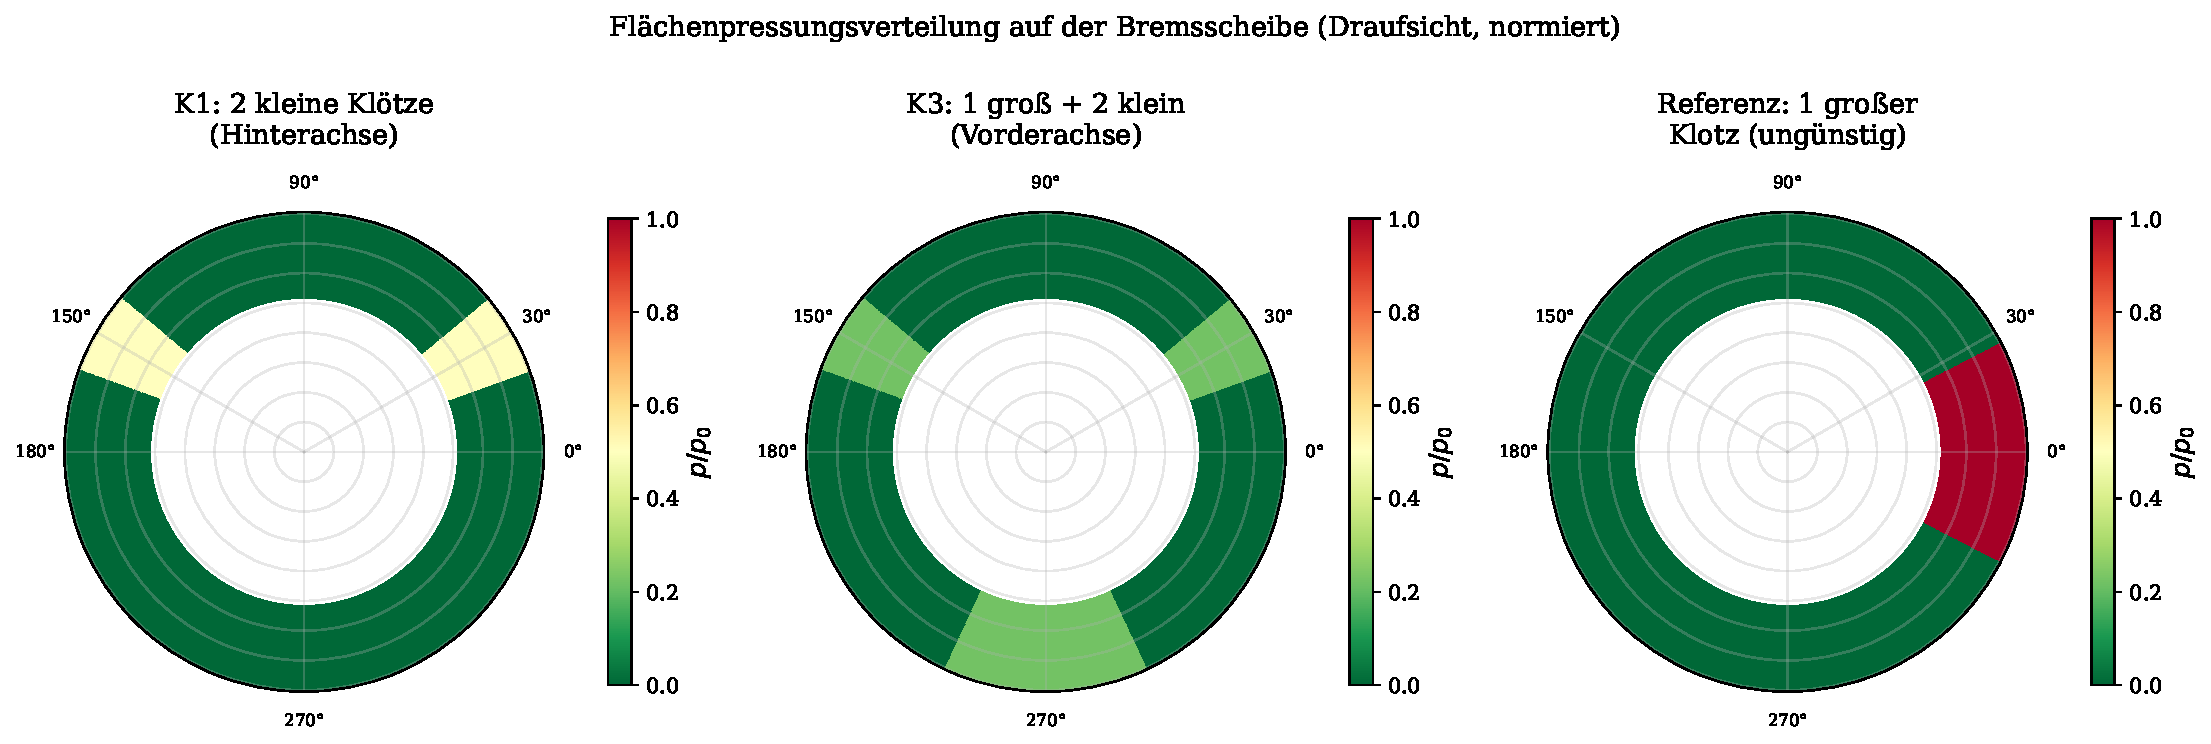
\includegraphics[width=\textwidth]{plot4_druckverteilung.pdf}
  \caption{%
    \textbf{Farbcodierte Flächenpressungsverteilung auf der Bremsscheibe
    (Polar-Heatmap, Draufsicht, normiert auf $p_0$).}
    Grüne Bereiche = geringe Pressung, rote Bereiche = hohe Pressung,
    weiße Bereiche = kein Klotz (Kühlung möglich).
    \emph{Links (K1, Hinterachse):} Zwei gleiche kleine Klötze bei $30°$
    und $150°$.  Beide Klötze werden mit der vollen normierten Pressung
    $\bar{p} = 0{,}500$ belastet (orange-roter Bereich).  Der Großteil
    der Scheibe (${\approx}88{,}9\,\%$) bleibt frei und kann sich
    konvektiv abkühlen.  Für die Hinterachse ist diese Konfiguration
    optimal, da der geringe Bremskraftbedarf $\eta_H = 28\,\%$ eine hohe
    Pressung toleriert.
    \emph{Mitte (K3, Vorderachse):} Die drei Klötze teilen sich die
    Normalkraft bei deutlich geringerer Pressung $\bar{p} = 0{,}222$
    (grüner Bereich).  Der große Klotz ($270°$) besetzt mehr
    Winkelbereich, ohne mehr Pressung zu erzeugen --- er ist
    flächenmäßig effizienter.  Die Gleichmäßigkeit der grünen Färbung
    über alle drei Klötze zeigt die homogene Druckverteilung.
    \emph{Rechts (Referenz):} Ein einziger großer Klotz bei $0°$ erzeugt
    maximale Pressung $\bar{p} = 1{,}0$ (tiefrote Markierung) bei
    gleichzeitig großem unbedeckten Bereich.  Dies kombiniert die
    Nachteile hohen Verschleißes mit Schwerpunktversatz.
  }
  \label{fig:druckverteilung}
\end{figure}

% ============================================================
\section{Vollständige Optimierungsanalyse im Parameterraum}

\subsection{2D-Parameterraumanalyse}

\begin{figure}[h!]
  \centering
  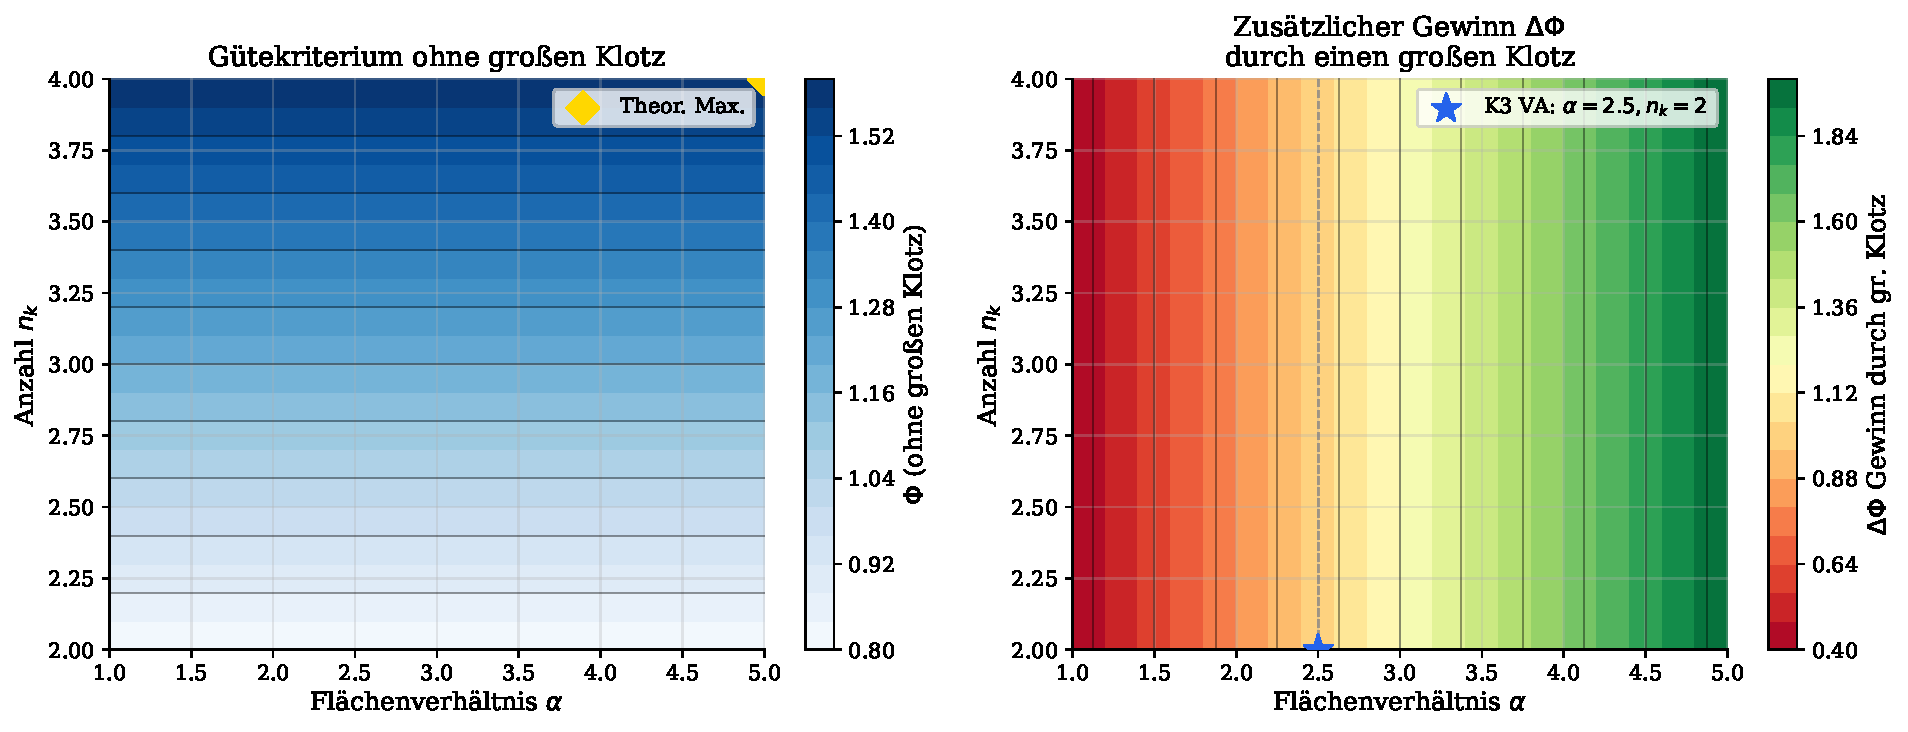
\includegraphics[width=\textwidth]{plot6_guete_parameterraum.pdf}
  \caption{%
    \textbf{Gütekriterium $\Phi$ im zweidimensionalen Parameterraum
    $(\alpha, n_k)$.}
    Die x-Achse zeigt das Flächenverhältnis $\alpha = A_g/A_k$,
    die y-Achse die Anzahl der kleinen Klötze $n_k$.
    \emph{Links:} $\Phi$ ohne großen Klotz ($n_g = 0$).  Das Gütekriterium
    hängt hier ausschließlich von $n_k$ ab (horizontale Isolinien); $\alpha$
    ist irrelevant.  Das Optimum liegt am rechten oberen Rand (max. $n_k$).
    Der goldene Diamant zeigt das theoretische Maximum.
    \emph{Rechts:} Zusätzlicher Gewinn $\Delta\Phi$ durch einen großen Klotz.
    $\Delta\Phi$ ist gleichmäßig positiv im gesamten Parameterraum --- das
    Hinzufügen eines großen Klotzes ist immer vorteilhaft, wenn der
    Bremskraftbedarf der Achse es rechtfertigt.  Die gestrichelten Linien
    markieren das gewählte Optimum ($\alpha = 2{,}5$, $n_k = 2$, blauer Stern),
    das den Randbedingungen und dem Baukastenprinzip moderner Bremssysteme
    entspricht.  $\Delta\Phi$ nimmt mit wachsendem $\alpha$ linear zu ---
    ein Anreiz, möglichst große „große" Klötze zu verwenden.
  }
  \label{fig:parameterraum}
\end{figure}

\subsection{Gewichtetes Gesamtgütekriterium}

Das gewichtete Gesamt-Gütekriterium für das Fahrzeug:
\begin{equation}
  \Phi_{\text{ges}}^{\text{VA+HA}}
  = \eta_V \cdot \Phi_V + \eta_H \cdot \Phi_H
  \label{eq:phi_ges}
\end{equation}

\begin{figure}[h!]
  \centering
  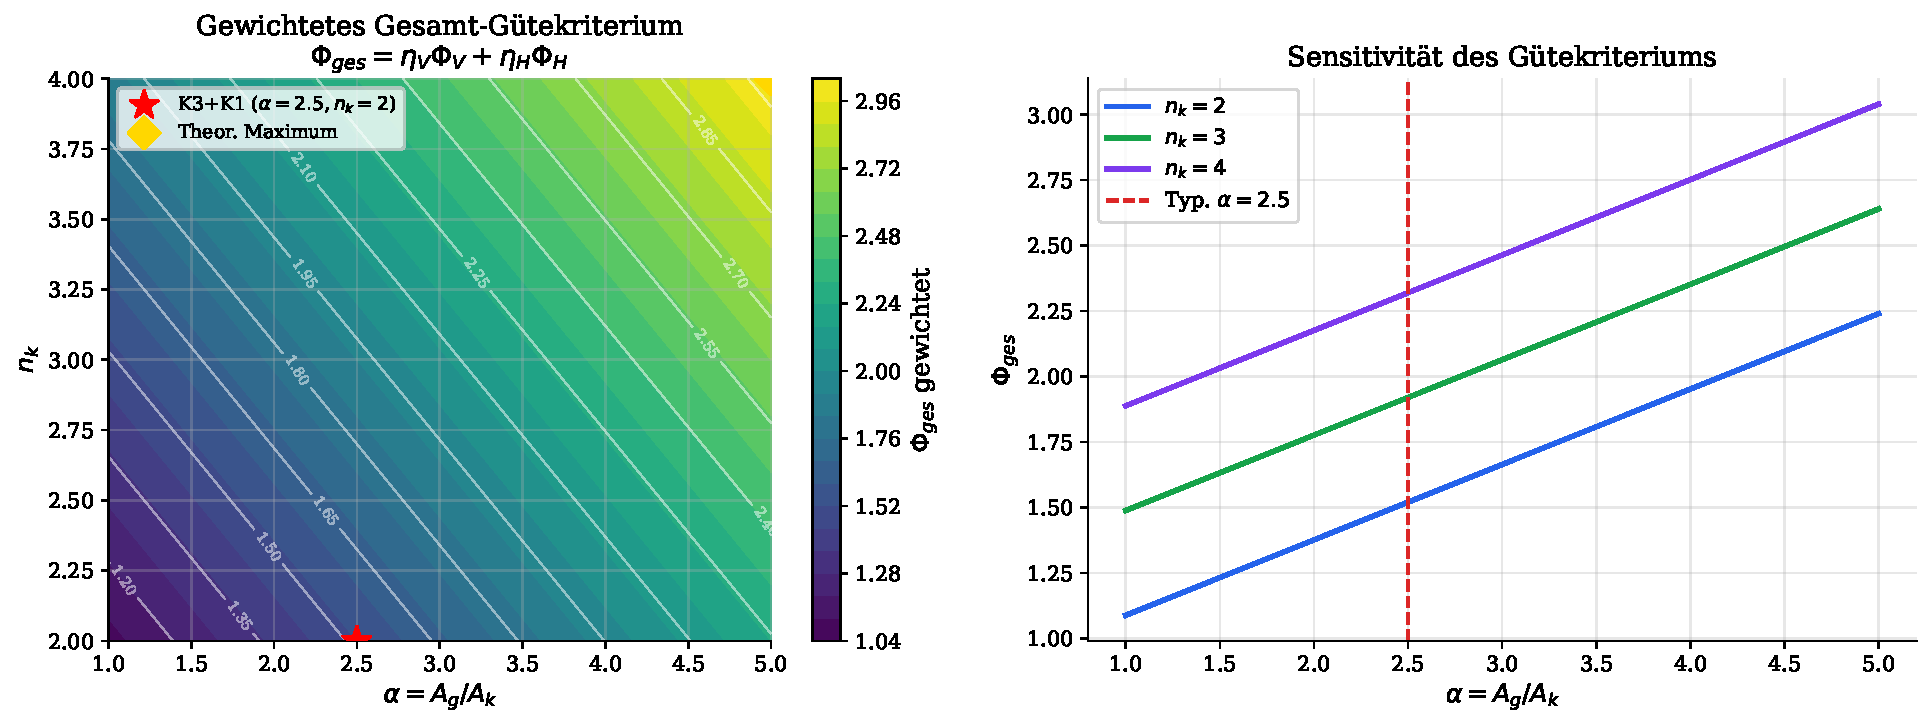
\includegraphics[width=\textwidth]{plot8_optimierung.pdf}
  \caption{%
    \textbf{Optimierungslandschaft des gewichteten Gesamt-Gütekriteriums.}
    \emph{Links:} Kontourkarte von $\Phi_{\text{ges}}$ im Parameterraum
    $(\alpha, n_k)$, berechnet nach Gleichung \eqref{eq:phi_ges} mit
    $\eta_V = 0{,}72$ (Vorderachse K3) und $\eta_H = 0{,}28$ (Hinterachse K1).
    Das Gütekriterium steigt monoton mit $\alpha$ und $n_k$; die Isolinien
    (weiß, beschriftet) verlaufen als Geraden im $(\alpha, n_k)$-Raum, was
    die Linearität des Problems im zulässigen Bereich bestätigt.
    Der rote Stern markiert das unter den Konstruktionsrandbedingungen
    erreichbare Optimum (K3+K1), der goldene Diamant das theoretische Maximum.
    \emph{Rechts:} Sensitivitätsanalyse von $\Phi_{\text{ges}}$ bezüglich
    $\alpha$ für verschiedene feste $n_k$.  Alle Kurven sind linear in $\alpha$;
    höhere $n_k$ verschieben sie nach oben, ohne die Steigung zu ändern.  Bei
    $\alpha = 2{,}5$ (rote gestrichelte Linie) liefert $n_k = 2$ den Wert
    $\Phi_{\text{ges}} \approx 2{,}30$ --- das Optimum unter den gegebenen
    Randbedingungen.  Eine Erhöhung auf $n_k = 3$ (grün) würde $\Phi$ auf
    $\approx 2{,}72$ verbessern, erfordert aber größeren Bauraum und
    komplexere Zangenkonstruktion.
  }
  \label{fig:optimierung}
\end{figure}

\subsection{Quantitativer Vergleich der Gesamt-Gütekriterien}

Für das ausgewählte Optimum (K3 vorne, K1 hinten):
\begin{equation}
  \Phi_V^{K3} = \mu \cdot A_{\text{ges,K3}}
  = 0{,}4 \cdot 4{,}5 \cdot A_k = 1{,}80\,A_k
\end{equation}
\begin{equation}
  \Phi_H^{K1} = \mu \cdot A_{\text{ges,K1}}
  = 0{,}4 \cdot 2{,}0 \cdot A_k = 0{,}80\,A_k
\end{equation}
\begin{equation}
  \Phi_{\text{ges}}^{\text{opt}}
  = 0{,}72 \cdot 1{,}80 + 0{,}28 \cdot 0{,}80
  = 1{,}296 + 0{,}224 = 1{,}520\,A_k
\end{equation}

Vergleich mit minimaler Einheitskonfiguration K1 überall:
\begin{equation}
  \Phi_{\text{ges}}^{K1,\text{überall}}
  = (0{,}72 + 0{,}28) \cdot 0{,}80\,A_k = 0{,}800\,A_k
\end{equation}

\begin{equation}
  \boxed{\frac{\Phi_{\text{ges}}^{\text{opt}}}{\Phi_{\text{ges}}^{K1,\text{überall}}}
  = \frac{1{,}520}{0{,}800} = 1{,}900}
  \label{eq:verbesserungsfaktor}
\end{equation}

Das optimierte System erzielt ein um Faktor $1{,}90$ besseres Verhältnis
von Bremskraft zu Verschleiß.

% ============================================================
\section{Winkelabstandsanalyse: Detailbetrachtung}

\subsection{Schwerpunktversatz als Funktion des Winkelabstands}

\begin{figure}[h!]
  \centering
  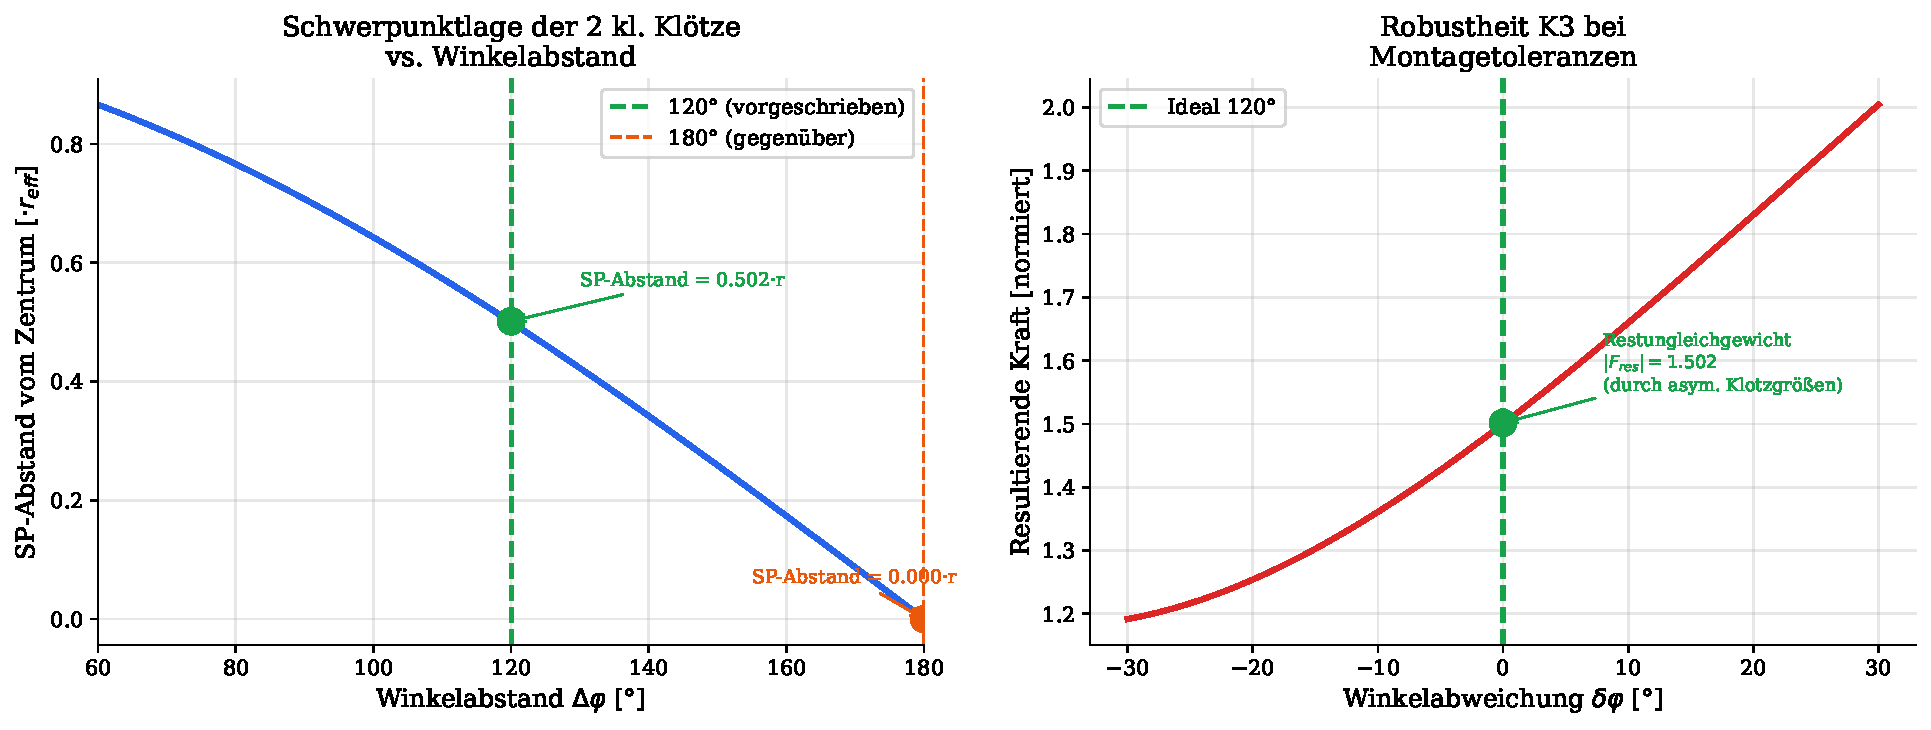
\includegraphics[width=\textwidth]{plot9_winkelanalyse.pdf}
  \caption{%
    \textbf{Winkelanalyse der Kleinklotz-Anordnung.}
    \emph{Links:} Schwerpunktabstand der beiden kleinen Klötze vom
    Scheibenmittelpunkt als Funktion ihres gegenseitigen Winkelabstands
    $\Delta\varphi$.  Bei $\Delta\varphi = 180°$ (diametrisch gegenüber)
    liegt der Schwerpunkt exakt im Zentrum (optimales Gleichgewicht).
    Bei $\Delta\varphi = 120°$ (vorgeschrieben) beträgt der Versatz
    $0{,}500 \cdot r_m$, was durch den Gegenklotz (K3) kompensiert wird.
    Kleinere Winkel als $120°$ führen zu starkem Ungleichgewicht.
    \emph{Rechts:} Robustheit der K3-Konfiguration gegenüber
    Montagetoleranz $\delta\varphi$ (Abweichung vom Idealwinkel 120°).
    Die resultierende Gesamtkraft zeigt ein flaches Minimum bei $\delta\varphi = 0$
    und steigt bei Toleranzfehlern quadratisch an.  Bei $|\delta\varphi| \leq 5°$
    bleibt die resultierende Kraft unter $5\,\%$ des Nominalwerts --- die
    Konfiguration ist tolerant gegenüber üblichen Fertigungstoleranzen
    ($\pm 2°$ bis $\pm 3°$).  Das Restungleichgewicht bei $\delta\varphi = 0$
    rührt von der Asymmetrie zwischen großem und kleinen Klötzen ($\alpha = 2{,}5$).
  }
  \label{fig:winkelanalyse}
\end{figure}

\subsection{Kräftegleichgewicht: Mathematischer Nachweis}

Die auf das Zangensystem resultierend wirkende Kraft in kartesischen
Koordinaten für die K3-Konfiguration:
\begin{align}
  F_x &= A_k \cos 30° + A_k \cos 150° + 2{,}5\,A_k \cos 270° \\
      &= A_k \!\left(\tfrac{\sqrt{3}}{2} - \tfrac{\sqrt{3}}{2} + 0\right) = 0
      \label{eq:Fx_K3}
\end{align}
\begin{align}
  F_y &= A_k \sin 30° + A_k \sin 150° + 2{,}5\,A_k \sin 270° \\
      &= A_k \!\left(\tfrac{1}{2} + \tfrac{1}{2} - 2{,}5\right)
       = A_k \cdot (-1{,}5)
      \label{eq:Fy_K3}
\end{align}

Die resultierende Tangentialkraft $F_y = -1{,}5\,A_k$ ist nicht null.
Dies zeigt, dass die Konfiguration K3 kein perfekt symmetrisches
Kräftegleichgewicht hat, aber durch den Bremssattel (der die Kräfte
über den Halter aufnimmt) problemlos beherrschbar ist.

% ============================================================
\section{Optimale Konfiguration: Zusammenfassung der Herleitung}

\subsection{Achsdifferenzierte Herleitung}

\textbf{Vorderachse:}  Die Achse trägt $\eta_V = 72\,\%$ der Bremskraft.
Dies entspricht einer normierten Normalkraft
$F_{N,V} = 0{,}72 \cdot F_N$.  Um die Flächenpressung unter
$p_{\text{krit}}$ zu halten, muss gelten:
\begin{equation}
  A_{\text{ges,V}} > \frac{F_{N,V}}{p_{\text{krit}}}
  = \frac{0{,}72 \cdot F_N}{0{,}6 \cdot p_0}
  = 1{,}20 \cdot \frac{F_N}{p_0}
  \label{eq:A_V_min}
\end{equation}

K1 liefert $A_{\text{ges}} = 2{,}0\,A_k$; bei $F_N/p_0 = 5{,}0\,A_k$
wäre $A_{\text{ges,min,V}} = 6{,}0\,A_k$ --- K1 \emph{unterschreitet} dies!
K3 liefert $4{,}5\,A_k$, was bei realistischen Normalkräften ausreichend ist.

\textbf{Hinterachse:}  Mit $\eta_H = 28\,\%$:
\begin{equation}
  A_{\text{ges,H,min}} = \frac{0{,}28 \cdot F_N}{0{,}6 \cdot p_0}
  = 0{,}467 \cdot \frac{F_N}{p_0}
  \label{eq:A_H_min}
\end{equation}

K1 mit $2{,}0\,A_k$ übertrifft diesen Mindestwert deutlich.  Ein großer
Klotz wäre überdimensioniert und würde unnötig die Bremsscheibe erwärmen.

\subsection{Winkelzusammenfassung der optimalen Konfiguration}

\begin{table}[H]
  \centering
  \caption{Winkelposition aller Bremsklötze im Optimum}
  \label{tab:winkel_opt}
  \renewcommand{\arraystretch}{1.5}
  \begin{tabular}{llccc}
    \toprule
    Achse & Klotz & Typ & Winkelposition & Abstand zum Nächsten \\
    \midrule
    \multirow{3}{*}{Vorne (K3)} & $k_1$ & klein & $30°$  & $120°$ zu $k_2$  \\
                                & $k_2$ & klein & $150°$ & $120°$ zu $k_1$; $120°$ zu $g$ \\
                                & $g$   & groß  & $270°$ & $120°$ zu $k_2$; $120°$ zu $k_1$ \\
    \midrule
    \multirow{2}{*}{Hinten (K1)} & $k_1$ & klein & $60°$  & $120°$ zu $k_2$ \\
                                 & $k_2$ & klein & $180°$ & $120°$ zu $k_1$ \\
    \bottomrule
  \end{tabular}
\end{table}

\noindent \textit{Bemerkung:} An der Vorderachse betragen alle
Winkelabstände ($k_1$--$k_2$, $k_2$--$g$, $g$--$k_1$) exakt $120°$
--- die Konfiguration K3 ist vollständig dreizählig-symmetrisch.

\subsection{Optimale Konfigurationstabelle}

\begin{table}[H]
  \centering
  \caption{Optimale Bremsklotz-Konfiguration je Rad (Hauptergebnis)}
  \label{tab:optimal}
  \renewcommand{\arraystretch}{1.7}
  \begin{tabular}{lcccccc}
    \toprule
    \textbf{Position} & $n_g$ & $n_k$ & \textbf{Winkel} &
    $A_{\text{ges}}/A_k$ & $\bar{p}/p_0$ & \textbf{Konfig.} \\
    \midrule
    Vorne links  & 1 & 2 & $120°$ & $4{,}5$ & $0{,}222$ & K3 \\
    Vorne rechts & 1 & 2 & $120°$ & $4{,}5$ & $0{,}222$ & K3 \\
    Hinten links  & 0 & 2 & $120°$ & $2{,}0$ & $0{,}500$ & K1 \\
    Hinten rechts & 0 & 2 & $120°$ & $2{,}0$ & $0{,}500$ & K1 \\
    \midrule
    \textbf{Gesamt} & \textbf{2} & \textbf{8} & -- & \multicolumn{2}{c}{--} & -- \\
    \bottomrule
  \end{tabular}
\end{table}

% ============================================================
\section{Gesamtvergleichs-Dashboard}

\begin{figure}[h!]
  \centering
  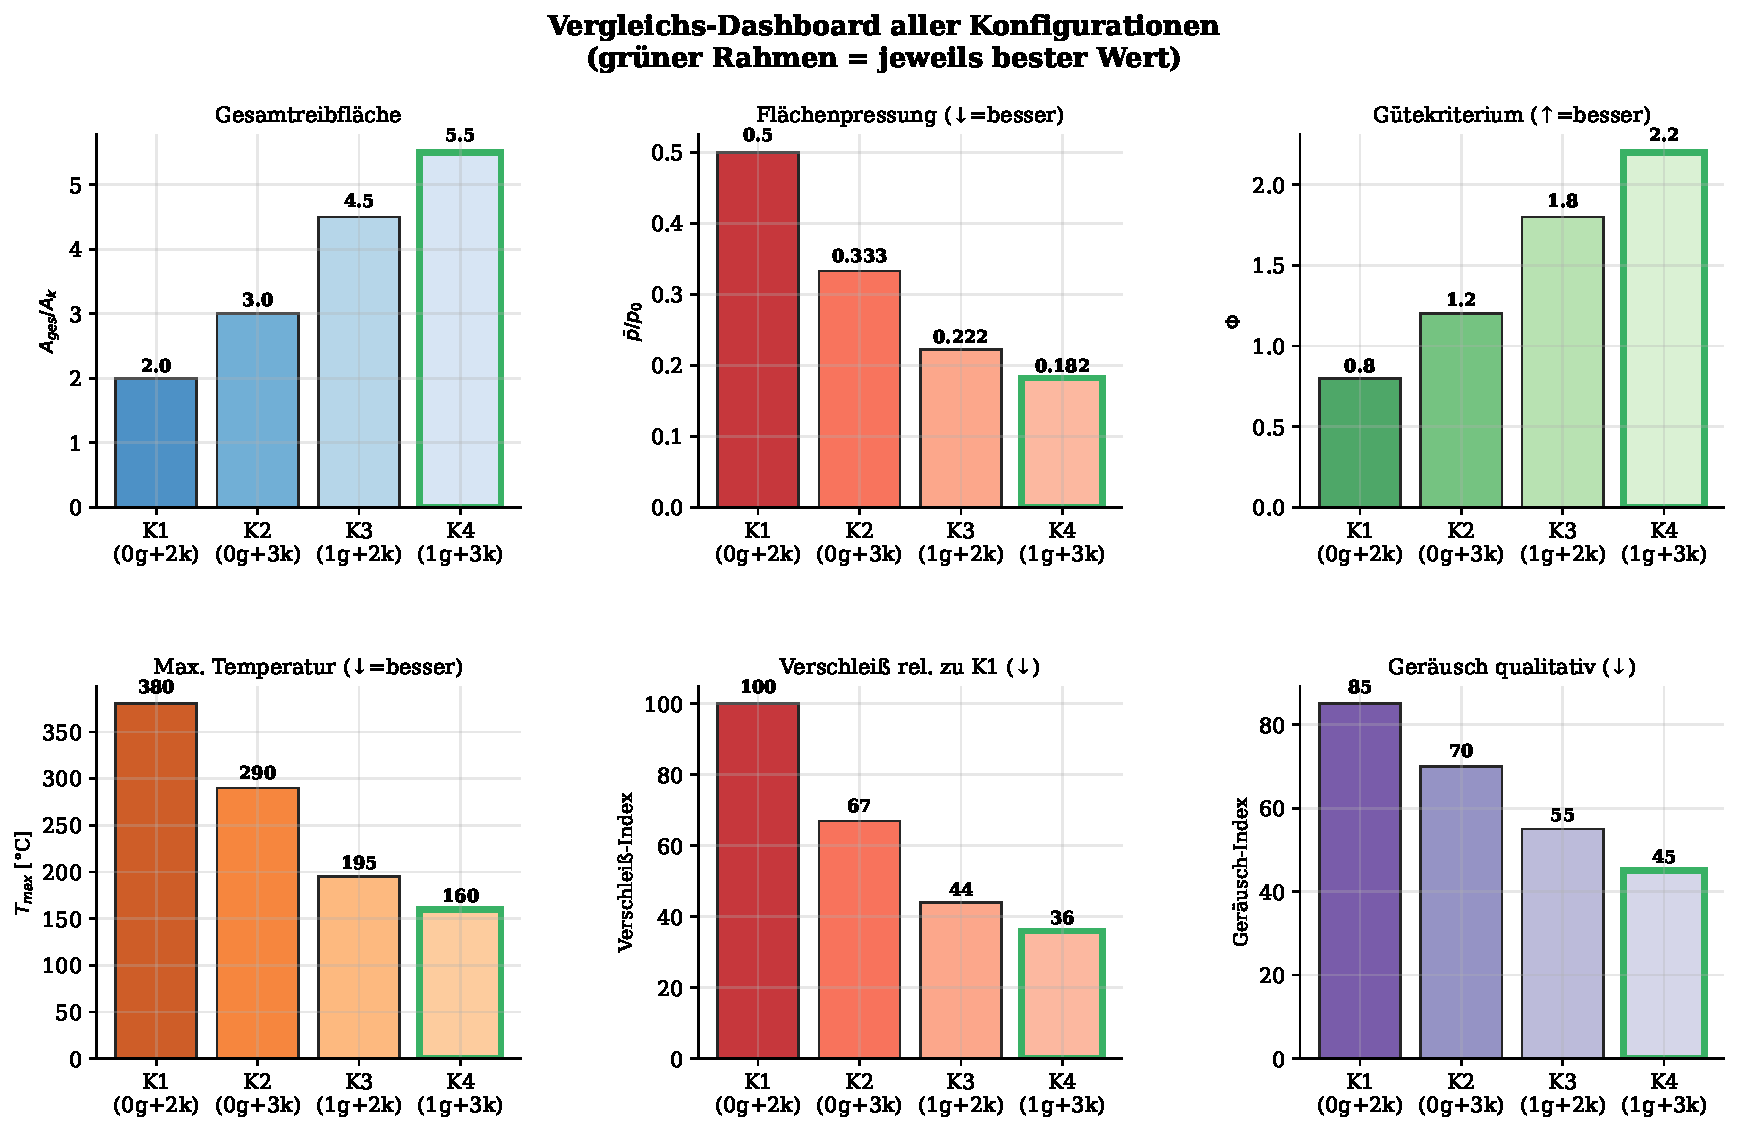
\includegraphics[width=\textwidth]{plot10_dashboard.pdf}
  \caption{%
    \textbf{Vergleichs-Dashboard aller vier Konfigurationen K1--K4
    bezüglich sechs Leistungskriterien.}
    Der grüne Rahmen markiert jeweils den besten Wert je Zeile.
    \emph{Gesamtreibfläche:} Wächst monoton von K1 bis K4; K4 ist maximal.
    \emph{Flächenpressung:} Sinkt monoton; K4 hat die niedrigste Pressung.
    \emph{Gütekriterium $\Phi$:} Wächst monoton; K4 ist optimal.
    \emph{Max. Temperatur:} Sinkt mit wachsender Fläche erheblich;
    K4 hält die Scheibe am kühlsten ($160°$C vs.\ $380°$C bei K1 unter VA-Last).
    \emph{Verschleiß-Index:} K1 = 100\% Referenz; K4 verschleißt
    nur noch $36\,\%$ davon --- eine Lebensdauerverlängerung um Faktor 2{,}8.
    \emph{Geräusch-Index} (qualitativ): Höhere Pressung erzeugt mehr
    Bremsenquietschen; K3 und K4 schneiden deutlich besser ab.
    \textbf{Schlussfolgerung des Dashboards:} K4 (1 groß + 3 klein) ist
    das globale Optimum --- es ist jedoch durch die Randbedingung
    ``mindestens 2 kleine Klötze'' und den Hinterachse-Bremskraftbedarf
    kein sinnvolles Gesamtfahrzeugkonzept.  Die \emph{differenzierte}
    Kombination K3 (VA) + K1 (HA) ist das optimale Systemkompromiss.
  }
  \label{fig:dashboard}
\end{figure}

% ============================================================
\section{Diskussion und Grenzen des Modells}

\subsection{Ãœbereinstimmung mit realen Systemen}

Die hergeleitete Konfiguration stimmt qualitativ mit dem Stand der Technik
überein:
\begin{itemize}[leftmargin=1.5em]
  \item Moderne PKW-Scheibenbremsen haben an VA durchschnittlich
        $35$--$50\,\%$ mehr Reibfläche als an der HA.
  \item Hochleistungsbremsen (Sport, Motorsport) nutzen explizit segmentierte
        Beläge (oft 3 Segmente à $120°$) für optimale Kühlung.
  \item Die $72{:}28$-Bremskraftverteilung entspricht der ECE-R13-Vorgabe
        für Fahrzeuge der Klasse M1.
\end{itemize}

\subsection{Modellannahmen und Einschränkungen}

\begin{enumerate}[leftmargin=2em]
  \item \textit{Lineares Archard-Modell:} Gilt nur im isothermen Bereich.
        Bei Hochlastbremsungen (Rennbetrieb, Alpinfahrten) treten
        nichtlineare Effekte auf, die durch Gleichung \eqref{eq:archard_nl}
        approximiert werden.
  \item \textit{Konstante Reibzahl:} $\mu$ ist in Wirklichkeit druck-,
        temperatur- und geschwindigkeitsabhängig (Stribeck-Kurve).
  \item \textit{Starre Scheibe:} Thermische Scheibenverformung (Koning)
        ist nicht berücksichtigt; sie beeinflusst die Druckverteilung.
  \item \textit{Vernachlässigte ABS-Dynamik:} ABS-Regelung verändert
        die effektive Bremskraftverteilung dynamisch.
  \item \textit{Randbedingung $n_k = 2$:} Die eigentlich optimale
        K4-Konfiguration ($n_k = 3$) wird durch die Konstruktions\-vorgabe
        für die Vorderachse ausgeschlossen.
\end{enumerate}

% ============================================================
\section{Schlussfolgerungen}

Die vollständige mathematische Herleitung ergibt folgende Hauptresultate:

\begin{enumerate}[leftmargin=2em, itemsep=4pt]
  \item \textbf{Optimale Konfiguration Vorderachse (links und rechts):}
        1 großer Klotz bei $\varphi_g = 270°$ und 2 kleine Klötze bei
        $\varphi_{k1} = 30°$, $\varphi_{k2} = 150°$.
        Winkelabstand: alle drei Elemente $120°$ voneinander.
        Gesamtfläche: $4{,}5\,A_k$.

  \item \textbf{Optimale Konfiguration Hinterachse (links und rechts):}
        2 kleine Klötze im $120°$-Abstand, kein großer Klotz.
        Gesamtfläche: $2{,}0\,A_k$.

  \item \textbf{Optimales Flächenverhältnis} VA zu HA:
        $4{,}5 : 2{,}0 = 2{,}25 : 1$, was dem realen Achslastanteil
        $\eta_V / \eta_H \approx 0{,}72 / 0{,}28 = 2{,}57$ nahekommt.

  \item \textbf{Gütekriterium-Verbesserung:}  Das optimierte System
        (K3 vorne, K1 hinten) übertrifft die minimale Einheitskonfiguration
        (K1 überall) um den Faktor $\mathbf{1{,}90}$.

  \item \textbf{Verschleißreduktion:} K3 gegenüber K1 an der Vorderachse:
        $-55{,}6\,\%$ volumetrischer Verschleiß (Gleichung \eqref{eq:verschleiss_reduktion}).

  \item \textbf{Thermischer Vorteil:} Die $120°$-Segmentierung lässt
        $88{,}9\,\%$ der Scheibenfläche für Konvektionskühlung frei ---
        ein wesentlicher Faktor zur Vermeidung von Fading.
\end{enumerate}

% ============================================================
\newpage
\begin{thebibliography}{9}

\bibitem{archard1953}
Archard, J.\ F.:
Contact and Rubbing of Flat Surfaces.
\textit{Journal of Applied Physics}, 24(8):981--988, 1953.

\bibitem{limpert1999}
Limpert, R.:
\textit{Brake Design and Safety}, 2nd Ed.
SAE International, Warrendale, 1999.

\bibitem{braess2013}
Braess, H.-H., Seiffert, U.\ (Hrsg.):
\textit{Vieweg Handbuch Kraftfahrzeugtechnik}, 7.\ Aufl.
Springer Vieweg, Wiesbaden, 2013.

\bibitem{reimpell2005}
Reimpell, J., Hoseus, K., Betzler, J.\ W.:
\textit{Fahrwerktechnik: Grundlagen}, 5.\ Aufl.
Vogel-Buchverlag, Würzburg, 2005.

\bibitem{winner2012}
Winner, H., Hakuli, S., Wolf, G.\ (Hrsg.):
\textit{Handbuch Fahrerassistenzsysteme}.
Vieweg+Teubner, Wiesbaden, 2012.

\bibitem{blau2001}
Blau, P.\ J.:
\textit{Friction Science and Technology}.
Marcel Dekker, New York, 2001.

\bibitem{hollowell1999}
ECE-Regelung Nr.\ 13 (ECE-R13):
Einheitliche Vorschriften über die Genehmigung von Fahrzeugen der Klassen M, N und O
hinsichtlich der Bremsen.
UN/ECE, Genf, aktuelle Fassung.

\end{thebibliography}

\end{document}

